\documentclass[presentation]{beamer}
\usepackage{../oop-slides-pianini}
\usepackage{url}
\setbeamertemplate{bibliography item}[text]
\author[Pianini]{Danilo Pianini\\Angelo Croatti, Simone Grotti, Mirko Viroli}
\title[L06 -- Advanced Collections]{06\\ Static code analysis, collezioni avanzate, enumeration e classi nested}

\begin{document}
	
\frame[label=coverpage]{\titlepage}

%====================
%Outline
%====================
\newcommand{\al}[0]{\textless}
\newcommand{\ar}[0]{\textgreater}
\newcommand{\gen}[1]{\al{}#1\ar{}}
\newcommand{\imgfr}[4]{\fr{#1}{#2
\begin{center}
\includegraphics[width=#3\textwidth]{#4}                    
\end{center}
}}

\section{JAR e gestione del classpath in Eclipse}

\begin{frame}[allowframebreaks]{Aggiunta di un jar al classpath di un progetto Eclipse}
	\begin{block}{}
		lab06 $\rightarrow$ Properties $\rightarrow$ Java build path $\rightarrow$ Libraries $\rightarrow$ Add Jar
	\end{block}
	\begin{center}
		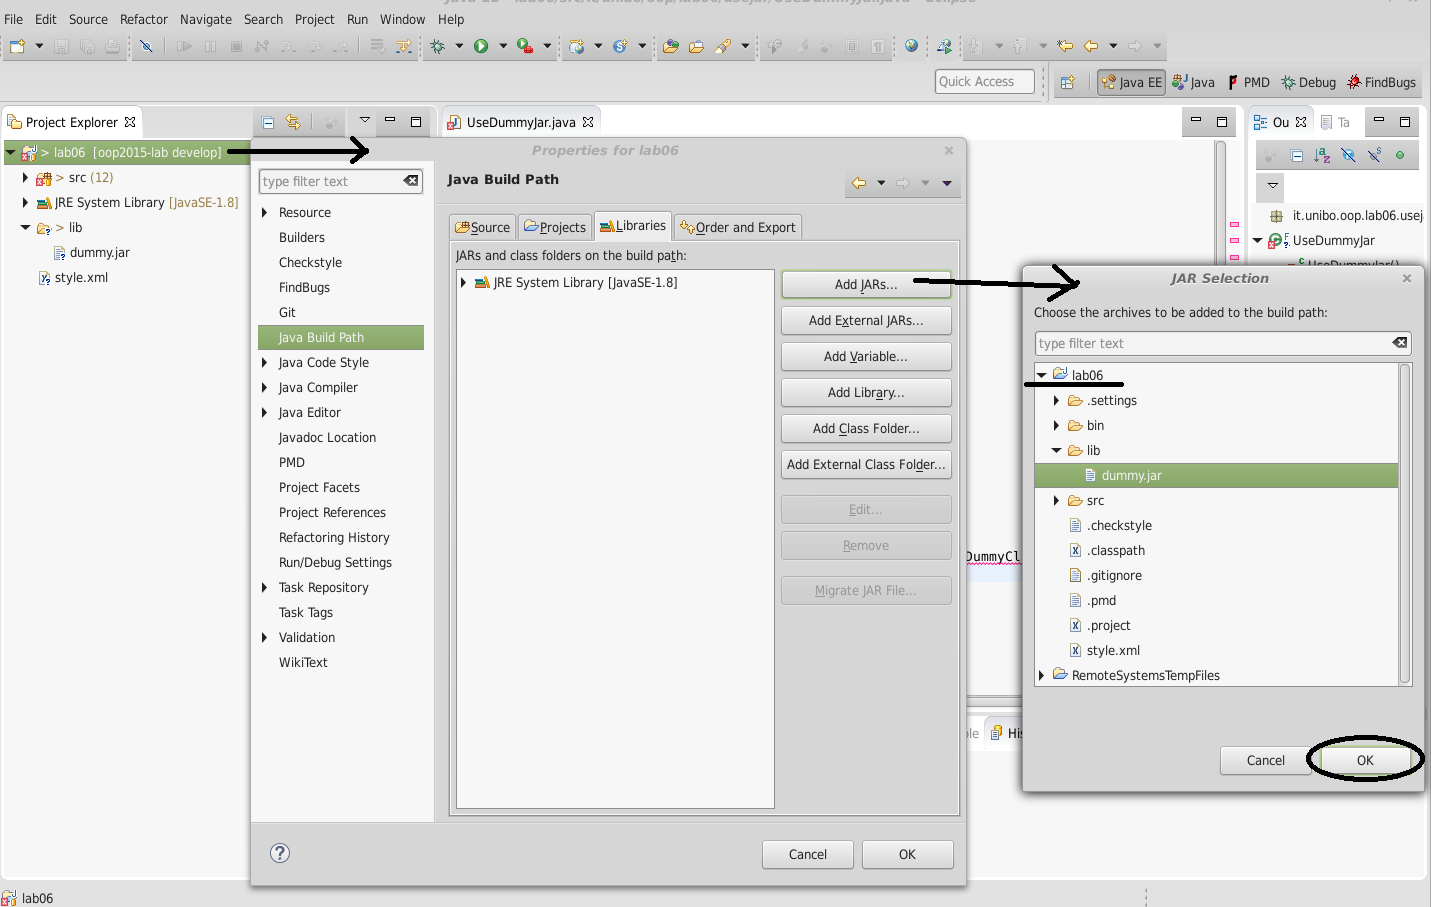
\includegraphics[width=0.82\textwidth]{img/addjar-1} \\
		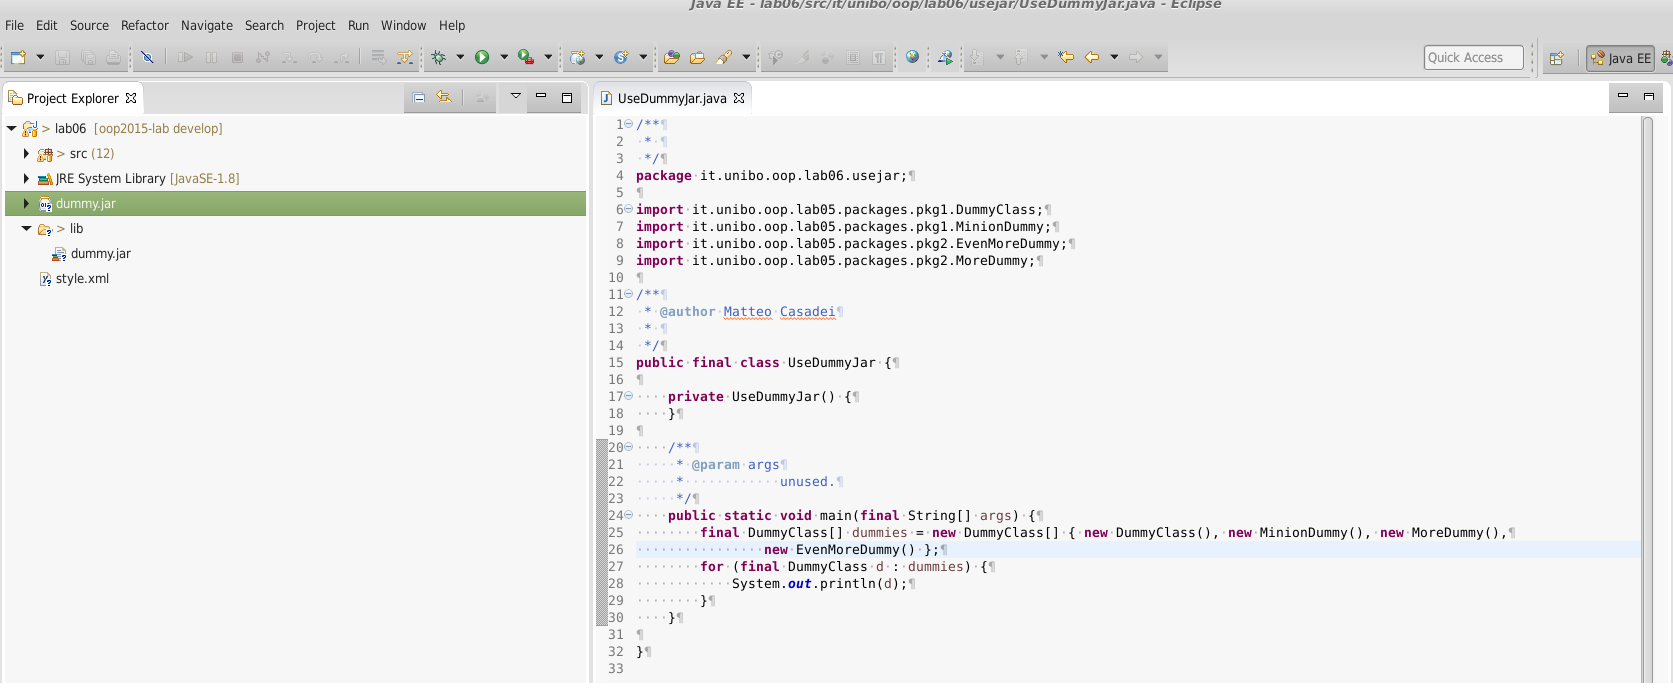
\includegraphics[width=0.99\textwidth]{img/addjar-2} \\
		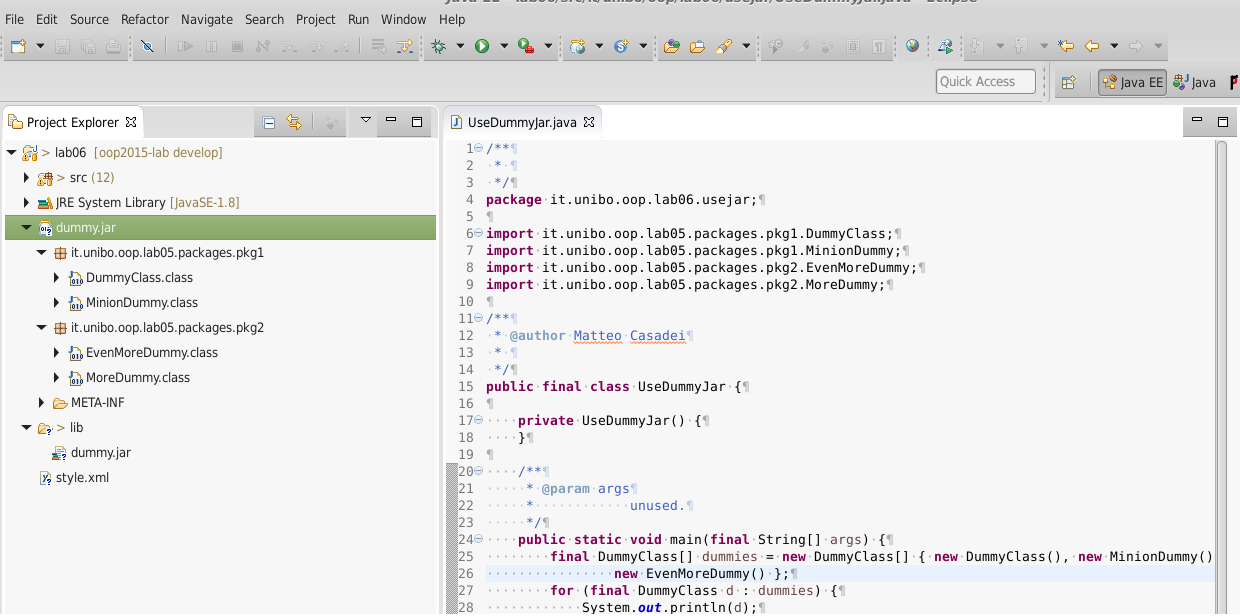
\includegraphics[width=0.99\textwidth]{img/addjar-3} \\
	\end{center}
\end{frame}

\section{Analisi di qualità del codice}

\begin{frame}{Analisi di qualità del codice sorgente}
	\begin{block}{Definizione}
		Software in grado di analizzare il codice sorgente per individuare:
		\begin{itemize}
			\item Potenziali bug, magari dovuti a distrazione
			\item Possibili miglioramenti, ottimizzazioni o pratiche difformi da quelle consigliate
			\item Codice duplicato, segnale di una progettazione discutibile
			\item Stile non conforme
		\end{itemize}
	\end{block}
	\begin{block}{Uso}
		L'analisi automatica del proprio codice garantisce sempre un elevata qualità del codice, aiuta ad apprendere il modo corretto di scrivere, riduce il costo di manutenzione e garantisce uniformità fra le parti sviluppate da persone diverse.
	\end{block}
\end{frame}


\begin{frame}[allowframebreaks]{Code checking}
	I software che vedremo sono eseguibili in due modalità\footnote{In realtà cominciano a prender piede anche servizi web come Codacy, ma non li tratteremo in questo corso...}:
	\begin{itemize}
		\item Stand-alone: il software viene eseguito e genera un report
		\item Come plug-in: il software viene integrato con l'IDE (nel nostro caso Eclipse), e segnala i problemi sotto forma di warning
	\end{itemize}
	Noi ci concentreremo nell'imparare la seconda modalità.
\end{frame}
\begin{frame}[allowframebreaks]{Code checkers in Eclipse}
	\begin{block}{Configurazione globale}
	La configurazione globale viene applicata a \textbf{tutti} i progetti del workspace, a meno che non sia sovrascritta localmente (non sempre è possibile).
		\begin{itemize}
			\item Veloce da configurare: si configura una volta, e i settaggi sono applicati su tutti i progetti
			\item Poco portabile: se inviamo il progetto ad un collaboratore, questi settaggi \textbf{non} saranno inviati: c'è il rischio di inconsistenze
			\item Ottimo da usare quando si hanno molti progetti nel workspace con la stessa configurazione, e si sviluppa da soli.
		\end{itemize}
	\end{block}
	\begin{block}{Configurazione locale}
	La configurazione locale va messa a punto singolarmente per ciascun progetto. Bisogna verificare che quella globale non la stia sovrascrivendo.
		\begin{itemize}
			\item Alta flessibilità: si possono specificare regole diverse per progetti diversi
			\item Alta portabilità: se si invia il progetto ad un collaboratore, questi settaggi vengono mantenuti
			\item Ottimo da usare quando si hanno pochi progetti, o ai progetti serve una configurazione diversa, oppure quando si lavora in modo collaborativo
		\end{itemize}
	\end{block}
	\begin{center}
		Noi faremo uso della configurazione \textbf{locale} \\
		\textbf{Voi farete} uso della configurazione locale nell'\textbf{elaborato finale}
	\end{center}

\end{frame}

\subsection{FindBugs}

\fr{FindBugs} {
  \bl{Cos'è} {
      FindBugs scansiona il bytecode generato dal compilatore, e dalla sua analisi cerca di scoprire potenziali bug nel sorgente, ad esempio:
      \iz {
        \item Uguaglianza esatta fra \texttt{float} o \texttt{double}
        \item Utilizzo di \texttt{==} invece di \texttt{equals()}
        \item Mancato retain a runtime di annotazioni
        \item Uso errato di meccanismi di sincronizzazione
        \item Vulnerabilità di sicurezza
        \item Tanti altri! Si veda: \url{http://findbugs.sourceforge.net/bugDescriptions.html}
      }
  }
}

\fr{FindBugs} {
	\bl{Plugin Eclipse} {
		Può essere installato dal marketplace di Eclipse cercando ``findbugs''.
		
		Una volta installato, apparirà un nuovo sotto-menu del progetto:
		
		\centering
		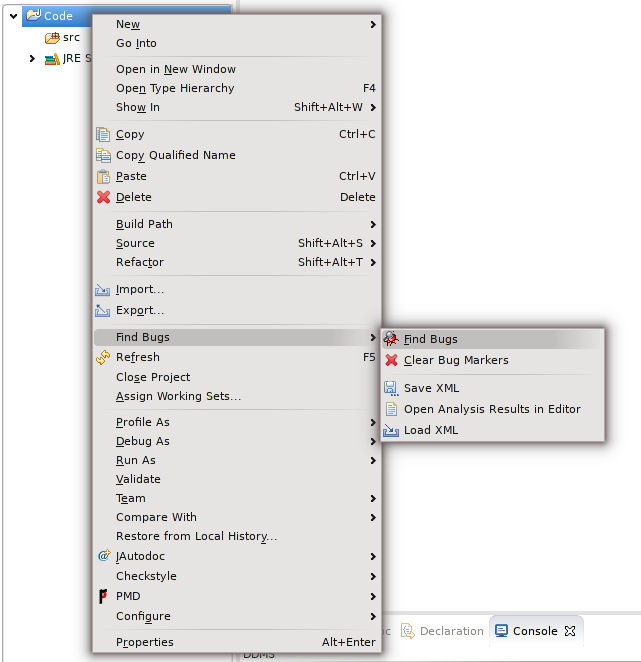
\includegraphics[width=0.5\textwidth]{img/findbugs}
	}
}

\fr{FindBugs --- Configurazione globale} {
	\centering
	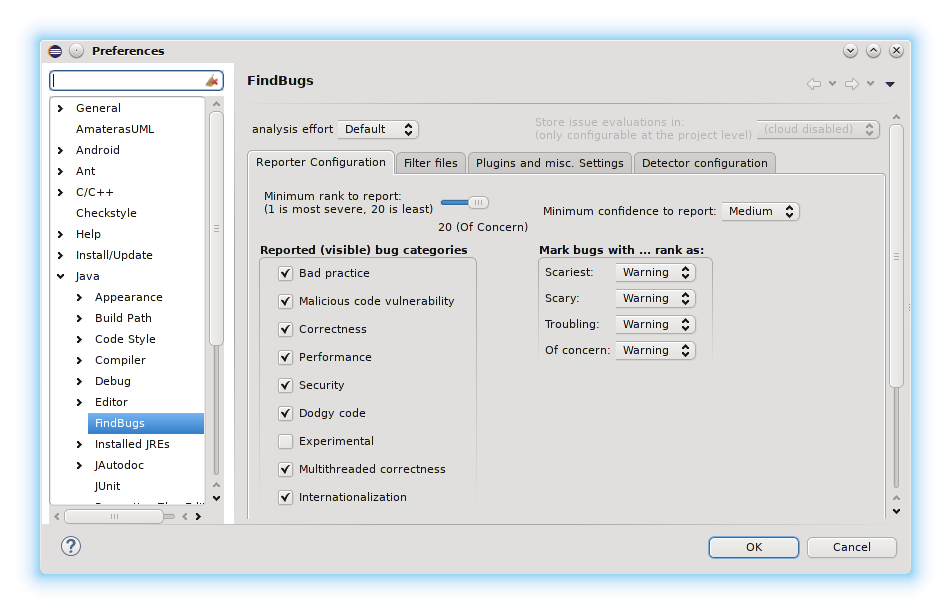
\includegraphics[width=0.99\textwidth]{img/findbugsconf}
}

\fr{FindBugs --- Configurazione del progetto} {
  In FindBugs, la configurazione locale \textbf{è più prioritaria} di quella globale.
  \centering
  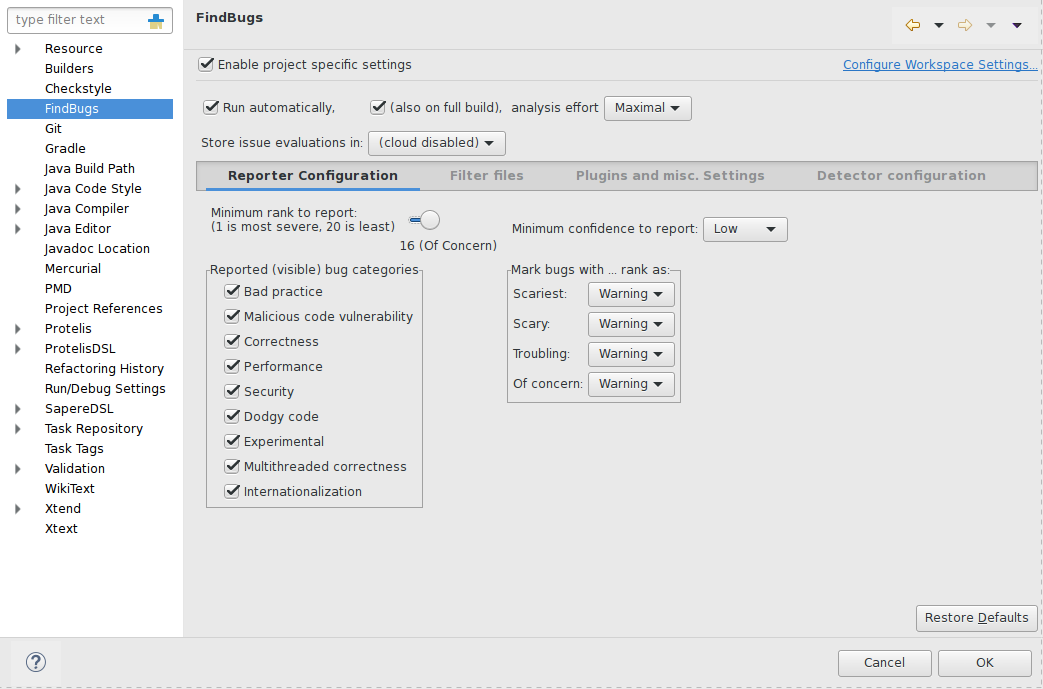
\includegraphics[width=0.9\textwidth]{img/findbugsproj}
}

\subsection{PMD e CPD}
\fr{PMD e CPD} {
	\bl{Cos'è} {
		PMD si occupa di trovare imperfezioni nel codice:
		\iz {
			\item Campi protetti o default
			\item Mancato uso di final
			\item Singular fields
			\item Usa CPD per verificare se vi siano blocchi di codice copincollati
			\item Tanti altri! Si veda: \url{http://pmd.sourceforge.net/pmd-4.3.0/rules/index.html}
		}
	}
}

\fr{PMD: Installazione} {
	\bl{Plugin Eclipse --- installazione} {
		Il marketplace contiene due plugin concorrenti: meglio eseguire l'installazione manuale.
		\iz {
			\item Dal menu Help, si selezioni ``Install new software''
			\item Si incolli l'indirizzo \url{https://sourceforge.net/projects/pmd/files/pmd-eclipse/update-site-latest/} e si prema Enter
			\item Si selezioni ``PMD for Eclipse 4''
			\item Next, Finish
			\item Si accetti il codice non firmato
			\item Si riavvii Eclipse come suggerito
		}
	}
	\bl{Plugin Eclipse} {
		Al termine dell'installazione, verrà installato un menu di opzioni globali, un menu di opzioni per progetto ed un menu contestuale.
	}
}

\fr{PMD --- Configurazione globale} {
	La configurazione di default di PMD contiene regole con limiti arbitrari, regole che hanno senso solo in particolari environment (e.g. J2EE) e regole controverse. È meglio rimuovere tali regole!
	\iz{
		\item Dalle proprietà di Eclipse, si allarghi il sotto menu PMD
		\item Si vada su Rule Configuration
		\item Si selezionino tutte le regole (click su una, poi ctrl+A)
		\item Si eliminino tutte le regole
		\item Si usi il tasto import
		\item Si importino (meglio per copia) le regole da un file XML
		\item Vi forniremo noi un buon file di regole!
	}
}

\fr{PMD --- Configurazione globale} {
	\centering
	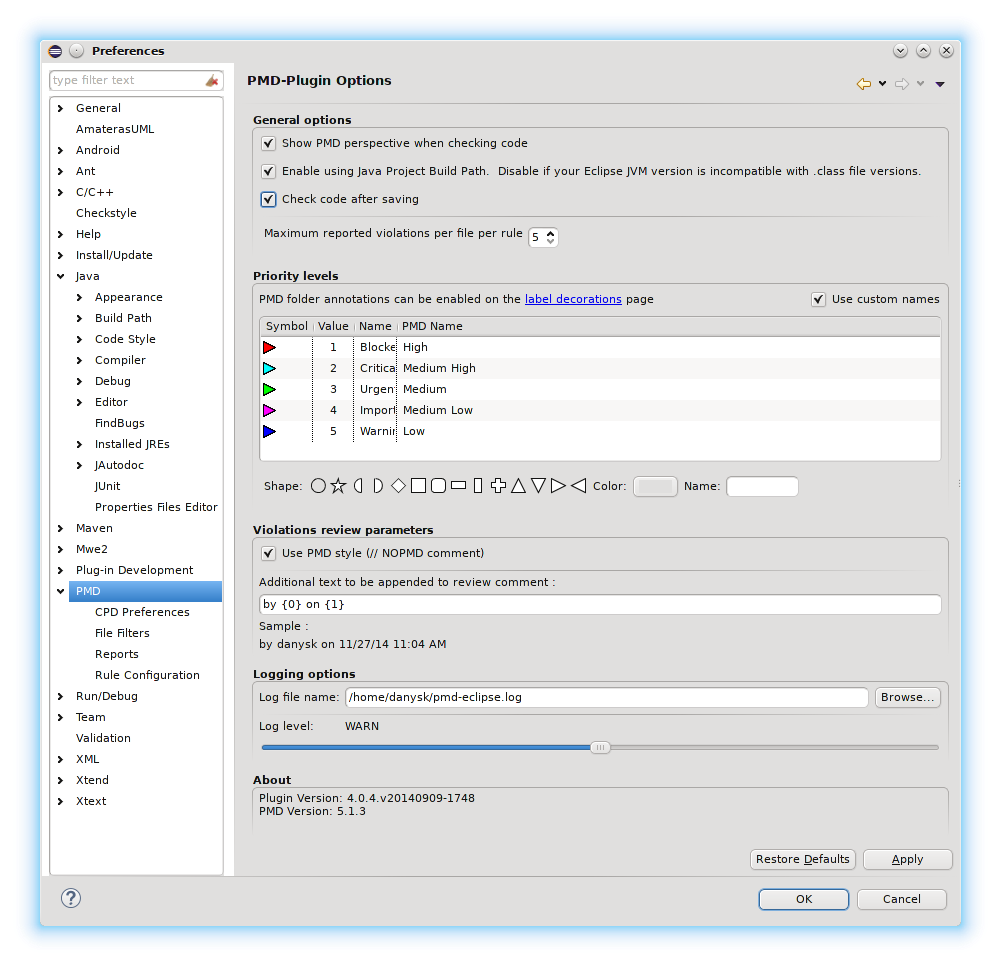
\includegraphics[width=0.75\textwidth]{img/pmdconf}
}

\fr{PMD --- Configurazione globale} {
  In PMD, la configurazione globale \textbf{sovrascrive} quella locale: disattivate ``Use global rule management'' se sviluppate un progetto su più sistemi
  \centering
  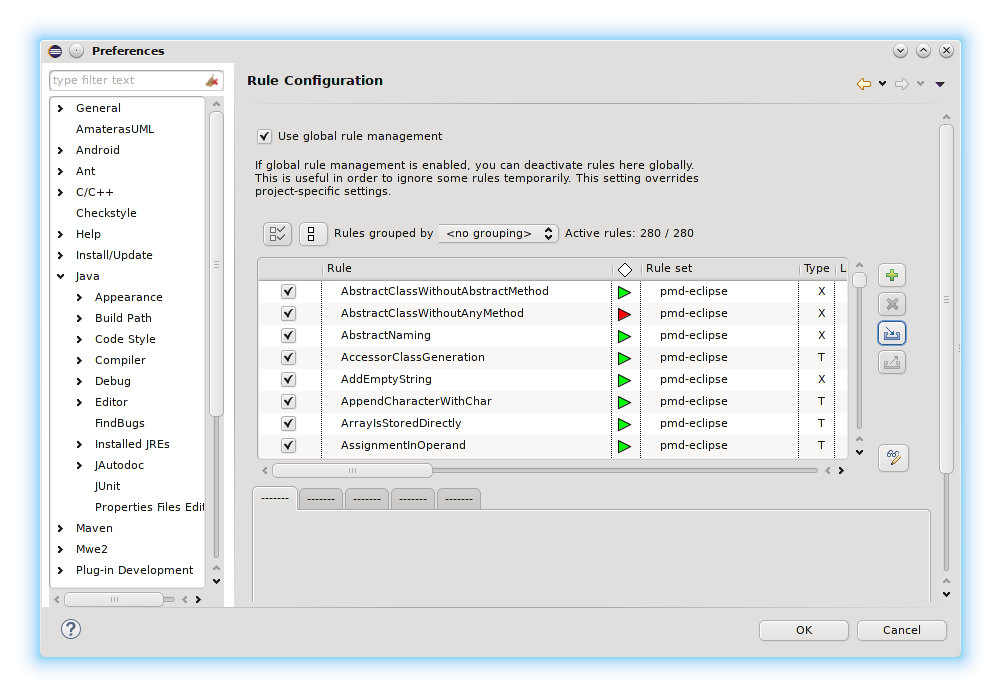
\includegraphics[width=0.9\textwidth]{img/pmdconf1}
}

\fr{PMD --- Configurazione globale} {
	\centering
	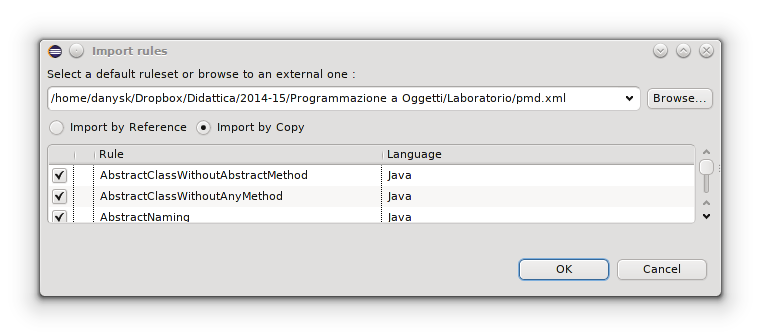
\includegraphics[width=0.99\textwidth]{img/pmdimport}
}

\fr{PMD --- Configurazione del progetto} {
	\textcolor{red}{ATTENZIONE}: Prima di attivare la configurazione locale, \textbf{assicurarsi} che il file pmd.xml sia stato copiato all'interno della cartella del progetto!
	\centering
	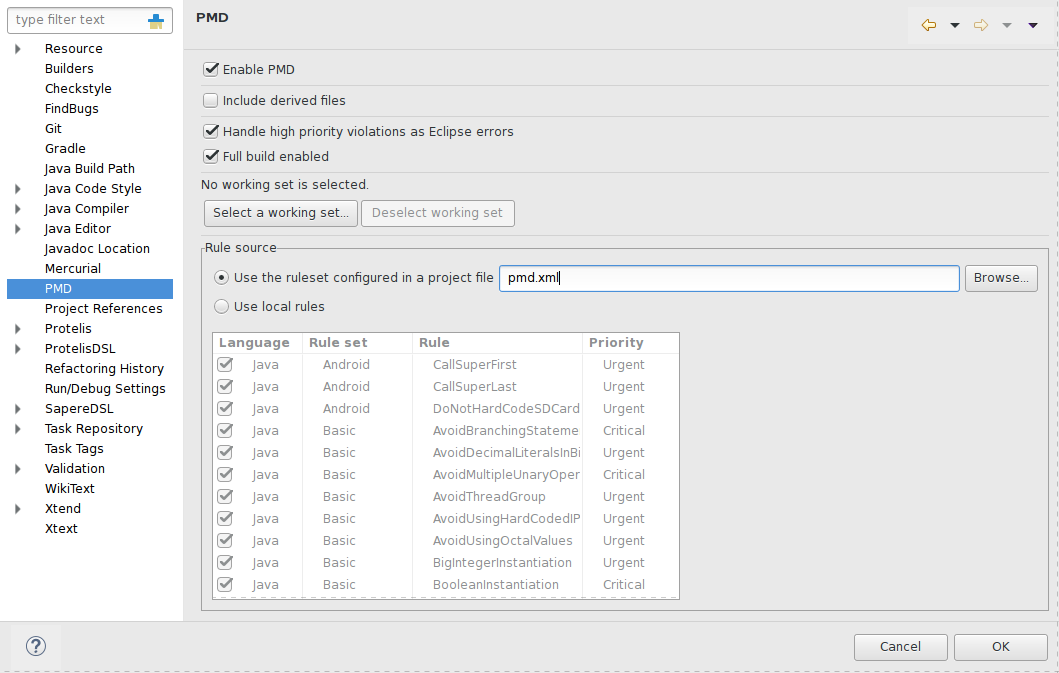
\includegraphics[width=0.9\textwidth]{img/pmdproj}
}


\subsection{Checkstyle}

\fr{Checkstyle} {
	\bl{Cos'è} {
		Checkstyle si occupa di trovare errori di stile:
		\iz {
			\item Mancanza di commento Javadoc
			\item Spaziature non corrette
			\item Parentesi assenti
			\item Magic numbers
			\item Altro: \url{http://checkstyle.sourceforge.net/checks.html}
		}
	}
}

\fr{Checkstyle} {
	\bl{Plugin Eclipse --- installazione} {
		Può essere installato dal marketplace di Eclipse cercando ``checkstyle''.
		
		\textcolor{red}{Attenzione}: il primo risultato potrebbe \textbf{non} essere quello corretto. Il logo corretto presenta la scritta ``eclipse-cs''.

		Al termine dell'installazione, verrà installato un menu di opzioni globali, un menu di opzioni per progetto ed un menu contestuale.
	}
}

\fr{Checkstyle --- Configurazione} {
	La configurazione di default di Checkstyle è eccessivamente pedante. Vi forniremo noi un file di configurazione idoneo:
	\en{
		\item Dalle proprietà di progetto, si clicki sul menu Checkstyle
		\item Si selezioni ``Local Check Configurations''
		\item Si scelga ``New''
		\item Si scelga ``Project Relative Configuration'' (mai usare path assoluti!)
		\item Utilizzando ``Browse...'' si punti al file di configurazione, che deve esser copiato nel progetto
		\item Si dia un nome e si prema ``OK''
		\item Si vada su ``Main''
		\item Si selezioni dal menu la nuova Check configuration
		\item Si attivi ``Checkstyle active for this project'' e ``Use simple configuration''
		\item ``OK''
	}
	\footnotesize
	Nota: la configurazione globale è molto simile, si ripetano gli step andando dal menu  Windows $\rightarrow$ Preferences $\rightarrow$ Java $\rightarrow$ Code style $\rightarrow$ Formatter 
}

\fr{Checkstyle --- Configurazione per-progetto} {
	\centering
	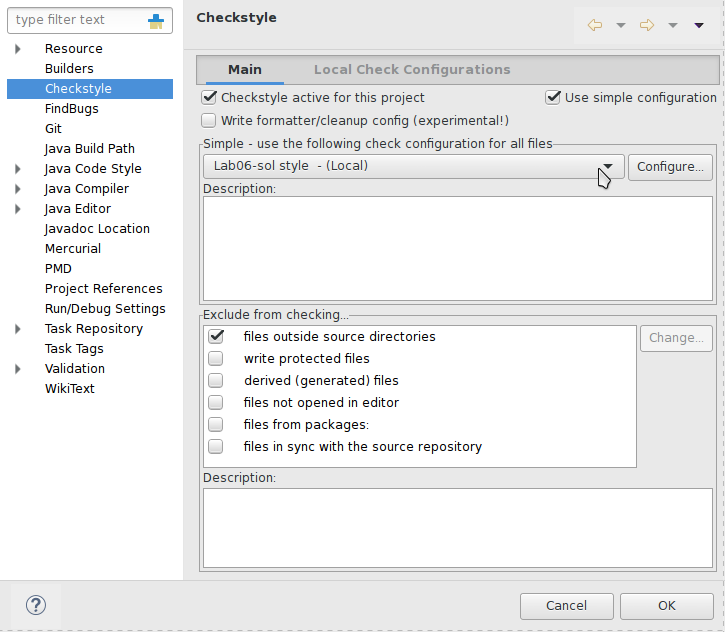
\includegraphics[width=0.7\textwidth]{img/checkstyle}
}

\section{Coding style: configurazione IDE Eclipse}
\fr{Configurare l'editor per una corretta formattazione del codice} {
	Checkstyle è in grado di supportarci nel verificare l'utilizzo di un corretto stile di codifica. Adattando le ``Java Code Convention'':
	\iz{
		\item 4 spazi per l'indentazione
		\begin{itemize}
			\item Nell'originale è consentito scegliere fra fra i due ed i quattro
		\end{itemize}
		\item Nessun carattere tab
		\begin{itemize}
			\item Nell'originale è consentito usarli
			\item Ma noi vogliamo indentazione consistente, quindi o spazi, oppure tab
			\item Essendo in JCC un tab equivalente ad 8 spazi, diventa troppo largo per una buona indentazione 
		\end{itemize}
		\item Linee lunghe al massimo 120 o 130 caratteri
		\begin{itemize}
			\item Nell'originale sono 80 per motivi storici (le schede perforate IBM avevano 80 colonne)
			\item Noi abbiamo i monitor, e anche i nostri colleghi
		\end{itemize}

	}
	\begin{block}{}
		Ora, però, dobbiamo configurare l'editor perché ci supporti nella scrittura di codice con lo stile corretto: come fare?
	\end{block}
}

\fr{Coding style: configurazione IDE Eclipse} {
	\centering
	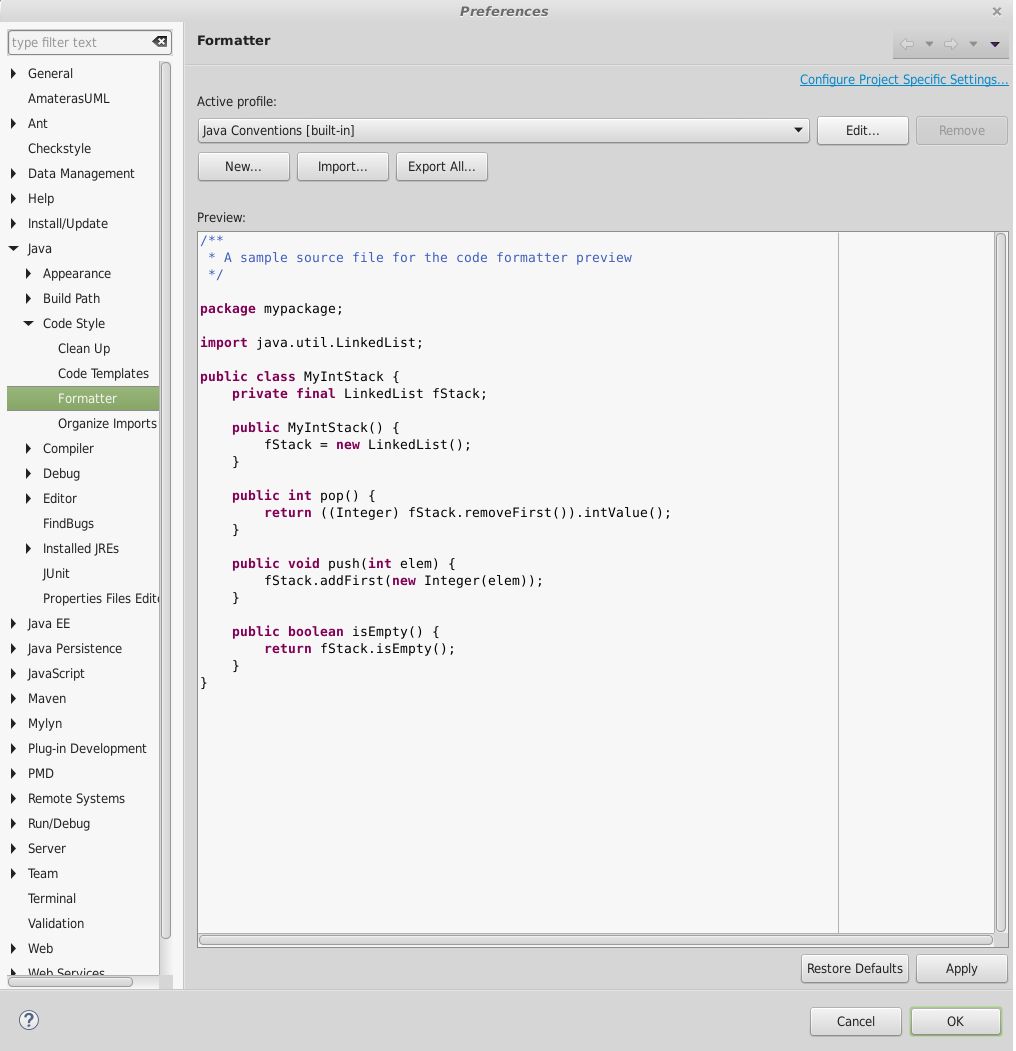
\includegraphics[width=0.99\textwidth]{img/ideconf-1}
}

\fr{Coding style: configurazione IDE Eclipse} {
	\centering
	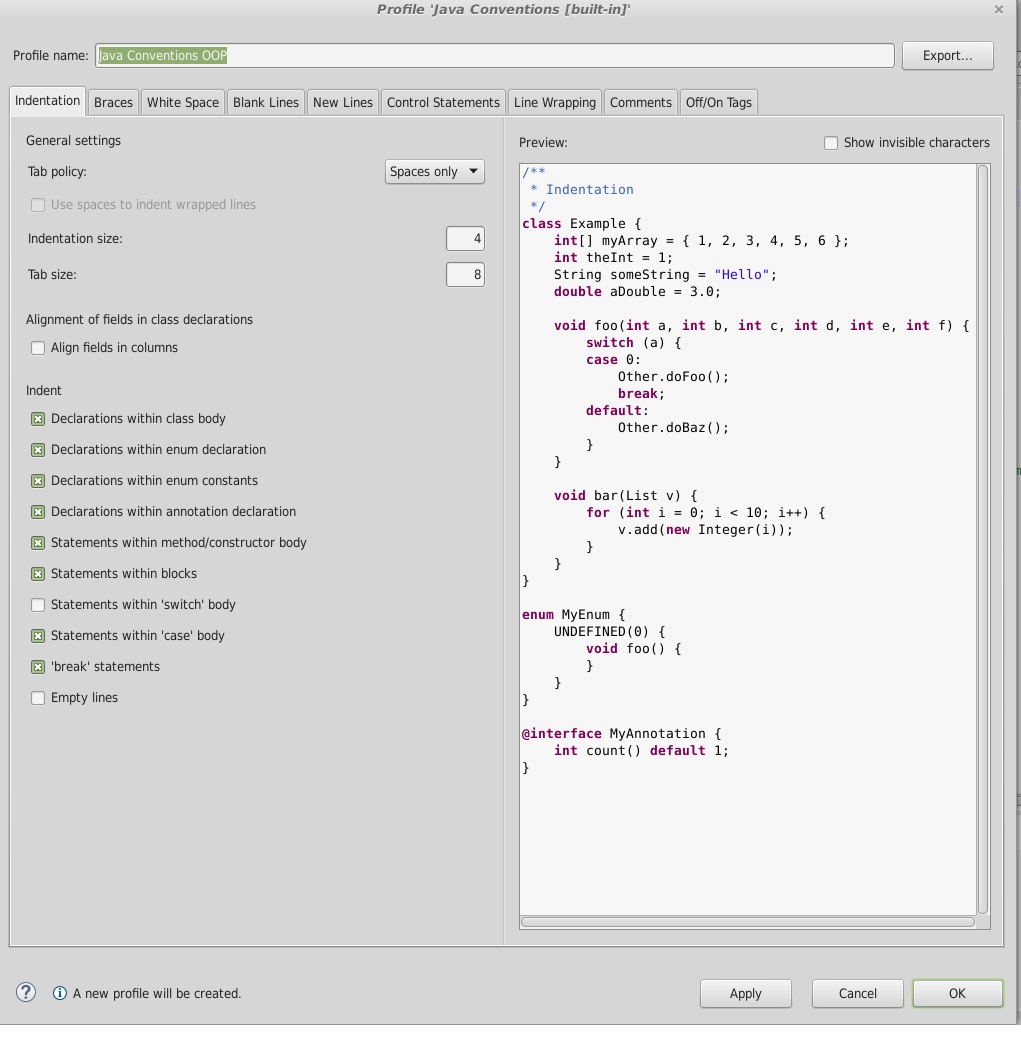
\includegraphics[width=0.99\textwidth]{img/ideconf-2}
}

\fr{Coding style: configurazione IDE Eclipse} {
	\centering
	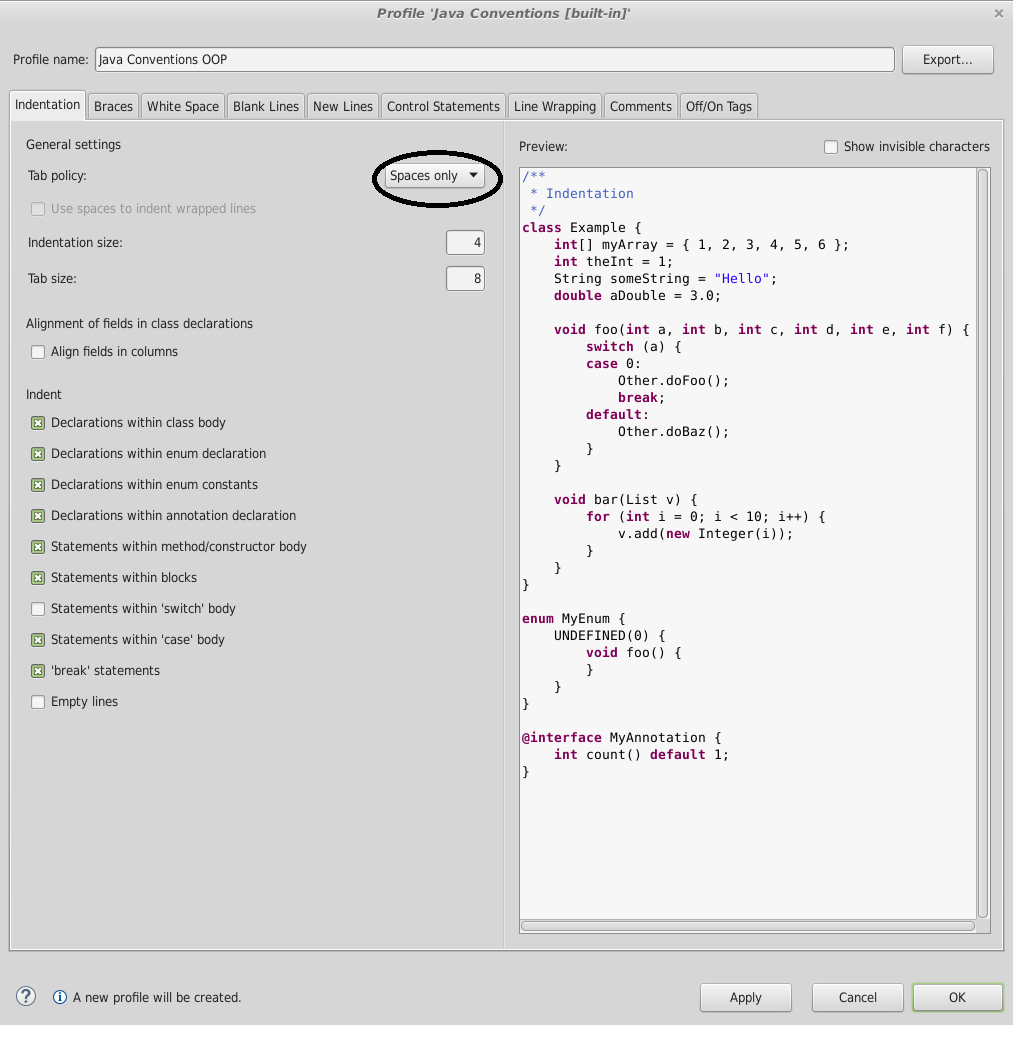
\includegraphics[width=0.99\textwidth]{img/ideconf-3}
}

\fr{Coding style: configurazione IDE Eclipse} {
	\centering
	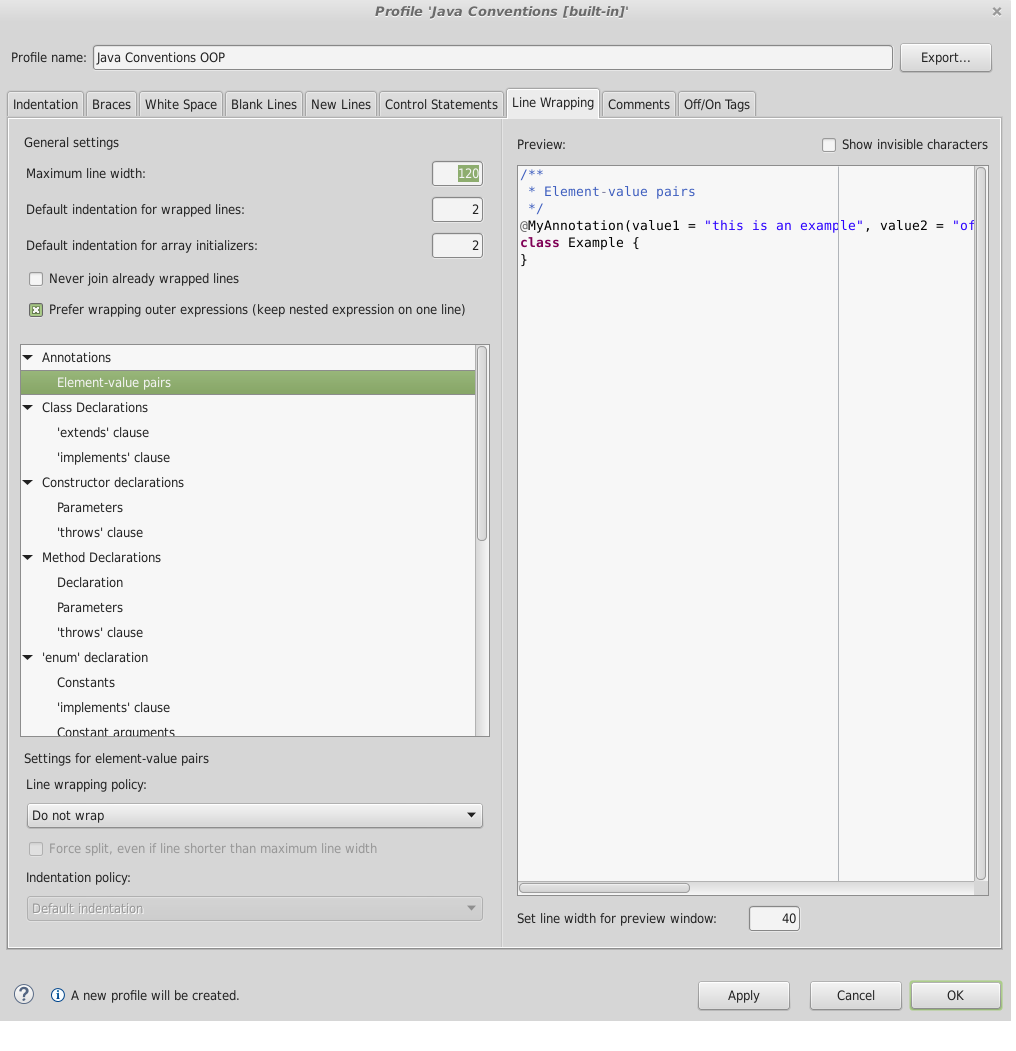
\includegraphics[width=0.99\textwidth]{img/ideconf-4}
}

\section{Esercitazione di oggi}

\fr{Modalità di Lavoro}{
  \bl{}{
    \en{
      \item Gli esercizi sono divisi in package con nomi progressivi
      \item Troverete un commento con le istruzioni per ciascun esercizio
      \item Risolvere l'esercizio in autonomia
      \item Cercare di risolvere autonomamente eventuali piccoli problemi che possono verificarsi durante lo svolgimento degli esercizi
      \item \textcolor{red}{Utilizzare le funzioni di test presenti nei sorgenti per il testing dell'esercizio}
      \item Contattare i docenti nel caso vi troviate a lungo bloccati nella risoluzione di uno specifico esercizio
      \item \textbf{A esercizio ultimato contattare i docenti per un rapido controllo della soluzione realizzata}
      \item Proseguire con l'esercizio seguente
       \item \textcolor{red}{Generare il file JAR dell'intera esercitazione} (o in lab o a casa in mancanza di tempo)
    }
  }
}


\end{document}

